\documentclass[../main/main.tex]{subfiles}
\begin{document}

\dominitoc
\faketableofcontents
\dominilof
\fakelistoffigures
\dominilot
\fakelistoftables

\chapter{Impact sur la cosmologie~: simulations}\label{ch:sims}
\epigraph{\openquote\textit{The Answer to the Great Question… Of Life, the
    Universe and Everything… Is… Forty-two.}\closequote}{Douglas \textsc{Adams},
    \textit{H2G2}}

Nous avons vu dans le chapitre précédent la manière dont \snana\ permettait de
traiter les biais et corrélations environnementales dans le calcul des
paramètres cosmologiques, et ainsi pourquoi son utilisation dans notre thèse
était pertinente.

Dans ce chapitre, nous présentons les simulations que nous avons effectuées avec
le logiciel. Dans un premier lieu, nous discutons des différentes corrélations
que nous avons testées \textit{via} l'utilisation de \hostlib\
(Section~\ref{sec:hpres}) et de la confection de nôtres
(Section~\ref{sec:hmake}). Par la suite, nous introduisons…

\vfill
\minitoc
\vfill

\newpage

\section{Présentation des \hostlib}\label{sec:hpres}

Dans sa forme la plus générale, une \hostlib\ ne possède pas de valeurs liées à
des paramètres de SNe~Ia (comme l'étirement ou la couleur)~; en effet, elle sert
originellement à utiliser le redshift photométrique de la galaxie hôte comme
valeur antérieure dans l'ajustement du redshift de la SN et à ajouter du bruit à
la SN simulée (voir Chapitre~\ref{ch:snana}). Avant d'intégrer notre modèle à
\snana, il nous a fallu reproduire les approches d'autres groupes utilisant le
logiciel. Nous avons choisi pour cela les études de~\cite{scolnic2016}, ci-après
SK\defcitealias{scolnic2016}{SK}, et de~\cite{popovic2021a}, ci-après
BP\defcitealias{popovic2021a}{BP}.

% However, the definition of a realistic model is the be questioned. In the
% pioneer work of \cite{scolnic2016}, there were no relationship between SNe and
% their host galaxy. \cite{popovic2021a} and~\cite{smith2020} introduced a link
% between the two thanks to a HOSTLIB: a table of 100,000 galaxies made to mimic
% the actual surveyed galaxies by the different samples. To each galaxy is
% associated a SN through its main fitted properties such as $x_1$ or $c$, which
% are generated by models of underlying distributions. Yet, this process was
% directed at guessing what relationship would fit more the data, by using bins of
% host galaxy masses and minimizing asymmetric Gaussian distributions for each in
% a backward-modeling way. It's a non-direct method to infer an evolution of an
% underlying distribution as a function of mass.
% 
% Our approach was to use independent data from the SNf sample that uses LsSFR to
% characterize a galaxy, as explained in Section~\ref{sec:model}, and make an
% evolving, analytical model that can then describe higher-redshift SNe in a
% forward-modeling approach. This method has the aim to be predictive and to
% better fit the data, as is discussed in Section~\ref{sec:results}. In order to
% implement our modeling in this framework, we had to modify the HOSTLIBs on which
% the simulations are based.

% SK16 is galaxy distribution from which you draw, P21 is a list with the
% distrubtion already in it, linking the relationships and $x_1$ and stuff
% already drawn. But there's no evolution in it, and we want to do that. Forward
% model that through.

% General, Brodie, us; no lightcurve fitting, and at the end of hostlib section
% w simulate antheon

% P21: There is a relationship, we'll try to guess it. Take data bns of mass,
% and calculate what the distribtion of stretch is for each. Looks differently
% in different bins: as a function of mass they have distribution. Backward
% models.  N21: our data is independent and we use it to show that it works on
% other data at higher redshift, is predictive, and involves an evolution of the
% distributions.

% Generate $z$, take closest $M$ entry in a table of host galaxies (HOSTLIB),
% then pick $x_1$, $c$ assuming underlying relationships defined by the BBC
% team.  Because we want to make these simulations with an evolving underlying
% distribution, we have to replace then $x_1$ values by what is estimated by our
% previous model.

\subsection{Étirement et couleur globales~: SK}\label{ssec:sk}

Dans leurs travaux, \citetalias{scolnic2016} n'incluent pas de lien d'étirement
ou de couleur avec les propriétés de la galaxie hôte mais uniquement une marche
de magnitude en fonction de sa masse $M_*$. Celle-ci est inclut dans les
\wgtmap\ des sondages, et est de \SI{0.05}{mag}. Le tirage des paramètres $x_1$
et $c$ se font alors depuis des distributions asymétriques Gaussiennes, une par
sondage simulé, décrites par~:
\begin{equation}\label{eq:skasym}
    P(p) = \left\{
        \begin{array}{l}
            e^{-\DS\frac{\abs{p-\mu}^2}{\sigma_-{}^2}
                \quad\text{si}\quad p\leq\mu} \\
            e^{-\DS\frac{\abs{p-\mu}^2}{\sigma_+{}^2}
                \quad\text{si}\quad p>\mu} \\
        \end{array}
        \right.
\end{equation}
avec $p = x_1$ ou $c$. Les valeurs des paramètres sont indiqués
Tableau~\ref{tab:skasym}.

\begin{table}[h]
    \centering
    \begin{threeparttable}
        \caption[Paramètres des distributions d'étirement et de couleur pour les
        simulations SK]{Paramètres des distributions sous-jacentes d'étirement
            et de couleur desquelles sont générées les SNe~Ia dans notre
        reproduction du travail de \citetalias{scolnic2016}.}
        \label{tab:skasym}
        \begin{tabular}{lcccccc}
            \toprule
            \multirow{2}[2]{*}{Sondage} &
            \multicolumn{3}{c}{$x_1$} &
            \multicolumn{3}{c}{$c$}\\
            \cmidrule(lr){2-4} \cmidrule(lr){5-7} &
            $\mu$ & $\sigma_-$ & $\sigma_+$ &
            $\mu$ & $\sigma_-$ & $\sigma_+$ \\
            \midrule
            PS1    &
            0,604  & 1,029 & 0,363   &
            -0,077 & 0,029 & 0,12\\
            SDSS   &
            1,141  & 1,653 & 0,100   &
            -0,038 & 0,048 & 0,079\\
            SNLS   &
            0,964  & 1,232 & 0,282   &
            -0,065 & 0,044 & 0,12\\
            LOWZ   &
            --     & --    & --      &
            -0,055 & 0,023 & 0,015\\
            \bottomrule
        \end{tabular}
        \begin{tablenotes}[flushleft]
        \item\small \textbf{\hspace{-3,2pt}Notes.} Les valeurs viennent du
            Tableau~1 de \citetalias{scolnic2016}, sauf pour LOWZ dont la
            distribution d'étirement est une double Gaussienne
            d'après~\cite{scolnic2018}.
        \end{tablenotes}
    \end{threeparttable}
\end{table}

Nous avons cependant utilisé les valeurs de paramètres de~\cite{scolnic2018}
pour la distribution d'étirement de LOWZ, qui est alors décrite par une
combinaison de deux Gaussiennes dont une asymétrique, telle que~:
\begin{equation}\label{eq:sklowz}
    P(x_1) = A_1\times
        \left\{
        \begin{array}{l}
            e^{-\DS\frac{\abs{x_1-\mu_1}^2}{\sigma_{-,1}{}^2}
                \quad\text{si}\quad x_1\leq\mu_1} \\
            e^{-\DS\frac{\abs{x_1-\mu_1}^2}{\sigma_{+,1}{}^2}
                \quad\text{si}\quad x_1>\mu_1} \\
        \end{array}
        \right. + A_2\times
        e^{-\DS\frac{\abs{x_1-\mu_2}^2}{\sigma_{2}{}^2}}
\end{equation}
Les valeurs sont indiquées Tableau~\ref{tab:sklowz} avec le rapport d'amplitude
$a=\frac{A_1}{A_2}$. 

\begin{table}[ht]
    \centering
    \begin{threeparttable}
        \caption[Paramètres de la distribution d'étirement pour l'échantillon
        LOWZ des simulations SK]{Paramètres de la distribution sous-jacente
            d'étirement pour l'échantillon LOWZ dans notre reproduction de
        l'étude de~\citetalias{scolnic2016}.}
        \label{tab:sklowz}
        \begin{tabular}{lcccccc}
            \toprule
            \multirow{2}[2]{*}{Sondage} &
            \multicolumn{6}{c}{$x_1$}\\
            \cmidrule(lr){2-7} &
            $\mu_1$ & $\sigma_{-,1}$ & $\sigma_{+,1}$ &
            $a$ &
            $\mu_2$ & $\sigma_{2}$ \\
            \midrule
            LOWZ &
            0,55 & 1,0 & 0,45  &
            0,55 &
            -1,5 & 0,5 \\
            \bottomrule
        \end{tabular}
        \begin{tablenotes}[flushleft]
        \item\small \textbf{\hspace{-3,2pt}Notes.} Les caractéristiques sont
            celles reportées dans l'annexe C de~\cite{scolnic2018}, mais les
            valeurs y étant erronées nous avons utilisé celles de l'équipe
            directement.
        \end{tablenotes}
    \end{threeparttable}
\end{table}

\subsection{Étirement et couleur selon la masse~: BP}\label{ssec:bp}

D'un autre côté, \citetalias{popovic2021a} définissent des distributions mères
Gaussiennes asymétriques pour $x_1$ et $c$ selon la masse de la galaxie hôte.
Ceci est effectué en découpant les données des sondages en intervalles selon
$M_*$~; dans chacun de ces intervalles sont déterminés les paramètres des
Gaussiennes asymétriques, puis à chaque entrée de la \hostlib\ sont sélectionnés
des paramètres d'étirement et de couleur selon la valeur de la masse de la
galaxie hôte. Ainsi, par rapport à SK, ces \hostlib\ présentent 2 colonnes
supplémentaires, une pour $x_1$ et une pour $c$, attribuant à chaque entrée une
valeur de ces paramètres à associer à la SN simulée. 

Ce procédé est réalisé pour LOWZ d'une part, menant à une \hostlib\ que nous
appelons «~BP\_lowz~», et pour la combinaison des sondages DES, SDSS, PS1 et
SNLS d'autre part, menant à une \hostlib\ que nous nommons «~BP\_highz~». Les
valeurs des paramètres correspondants sont disponibles dans l'annexe A2
de~\citetalias{popovic2021a}.

Ce sont ces \hostlib\ qui constituent la base de notre étude~; en réalité, les
\hostlib\ SK sont celles de BP où nous avons retiré le tirage des colonnes $x_1$
et $c$.

\subsection{Étirement selon l'âge~: NN}\label{ssec:nn}

Notre approche des corrélations entre environnement et supernova est une
variation forte par rapport aux précédentes implémentations, puisqu'elle résulte
d'une modélisation prospective plutôt que purement phénoménologique. Pour notre
étude, nous avons besoin de relier l'étirement attribué à la SN avec l'âge de
son environnement, en correspondance avec nos travaux précédents
\citep[][ci-après NN]{nicolas2021}\defcitealias{nicolas2021}{NN}. Nous
augmentons donc les \hostlib\ en faisant correspondre un âge à chaque entrée des
tables~; ainsi, par rapport aux \hostlib\ BP, nous avons donc une colonne
indiquant si la SN est jeune ou vieille, et nommons ces \hostlib\ «~NN~». La
réalisation de cette \hostlib\ est présentée dans la Section~\ref{sec:hmake}.

\subsection{Étirement et marche de magnitude selon l'âge~: NR}\label{ssec:nr}

Comme nous l'avons vu précédemment, l'âge des SNe~Ia a une double implication~:
celle de l'évolution de la distribution sous-jacente de l'étirement avec le
redshift (Chapitre~\ref{ch:stretch}), mais aussi une marche de magnitude de
$\gamma_{\rm env} = \SI{0,13}{mag}$ entre les SNe~Ia jeunes et vieilles
\citep[Chapitre~\ref{ch:stretch},][]{rigault2020}. Nous avons implémenté cette
valeur à la place de la marche de magnitude selon $M_*$ incluse dans les
\wgtmap\ des sondages \textit{via} l'ajout d'une colonne donnant une variation
de magnitude de $\pm\SI{0.065}{mag}$ aux \hostlib\ NN~: ces nouvelles \hostlib\
se nomment «~NR~» pour «~\textsc{Nicolas} \textsc{Rigault}~», et présentent
l'exacte même colonne d'étirement que les NN.

\section{Confection des \hostlib\ NN et NR}\label{sec:hmake}

Afin de simuler des SNe~Ia avec notre modèle, que ce soit pour NN ou NR, nous
avons besoin que les propriétés des galaxies hôtes suivent les distributions de
ce qui a été observé par les différents sondages simulés. Bien que nous
soutenions que le LsSFR est un meilleur traceur de l'environnement d'une SN
\citep{briday2022}, la plupart des sondages caractérisent les galaxies avec leur
masse stellaire. Étant donné que le LsSFR repose sur la masse de la galaxie
hôte\footnote{pour rappel~: $\mathrm{sSFR} = \frac{\rm SFR}{M_*}$}, nous ne
pouvons pas uniquement nous baser sur la valeur du redshift $z$ d'une entrée des
\hostlib\ BP pour y assigner un étirement. Nous attendons effectivement que les
galaxies vers $M_*\approx12$ ne contiennent des SNe~Ia vieilles  alors que les
galaxies de $M \gtrsim 7$ n'en contiennent que des jeunes.

Par conséquent, afin de comparer les implications de notre modélisation basée
sur le LsSFR avec ce que les autres sondages ont observé, nous avons dû
modéliser les masses des galaxies hôtes par rapport au LsSFR~; nous avons pour
cela utilisé le même échantillon du Chapitre~\ref{ch:sample} que pour la
modélisation de l'étirement du Chapitre~\ref{ch:stretch}. Cependant, nous
soulignons que cette étude n'a pas pour volonté de décrire l'évolution des
masses des galaxies hôtes (qui sont des propriétés globales) avec le LsSFR d'une
supernova (étant une propriété intrinsèque de celles-ci)~: son utilité est
d'associer de manière cohérente un âge à une SN caractérisée par un certain
redshift et par une masse de galaxie hôte.

\subsection{Modélisation du lien entre masse et redshift}\label{ssec:mmod}

De la même manière que dans le Chapitre~\ref{ch:stretch}, nous utilisons le
LsSFR comme traceur de l'âge d'une SN, mais cette fois sur les estimations de
masse du sondage SNf. Ensuite nous modélisons les populations jeune et vieille
par une série de paramétrisations différentes et choisissons celle qui a le plus
faible AIC. Cependant, les masses SNf ont été calculées à l'aide de l'Équation~8
de~\cite{taylor2011} (voir~\cite{rigault2020}) alors que d'autres études du
catalogue Pantheon utilisent différentes techniques d'estimation de la masse qui
pourraient donner des valeurs de sortie différentes pour une même galaxie.

L'estimation de \textsc{Taylor} utilise la magnitude AB absolue en bande $i$
d'une galaxie, $M_i$. Elle est déduite de la magnitude apparente $m_i$
connaissant le redshift de la galaxie mais suppose que la bande $i$ observée est
proche de celle du référentiel de repos, ce qui est vrai pour les redshift de
SNf qui sont inférieurs à $z\approx 0,05$. Les relevés de l'échantillon Pantheon
sont à des redshifts plus élevés et ont utilisé un ajustement des distributions
spectrales d'énergie (en anglais SED pour \textit{spectral energy
distributions}) des galaxies pour éviter les corrections K dans cette procédure.

Nous avons appliqué la même analyse à l'échantillon SNf~; les données ainsi
calculées sont nommées «~SEDSNf~» par la suite, et l'échantillon fiduciel
utilisant SEDSNf est nommé «~SED fiduciel~». À cause de l'absence de 4 galaxies
hôtes dans les catalogues de données nécessaires à ce calcul, l'échantillon
SEDSNf est réduit à 110 données, au lien de 114 pour SNf. Nous indiquons
également que nous nous limitons pour cette étude aux galaxies de $M_* >
10^7\si{\Msun}$, étant donné que les valeurs inférieures servent à indiquer
qu'aucune galaxie hôte n'a été définie~; l'échantillon fiduciel tombe alors à
548 données, et SED Fiduciel à 544.

Nous avons donc réalisé cette étude de l'évolution des distributions
sous-jacentes de masse avec le LsSFR en utilisant~:
\begin{enumerate}
    \item [\bfseries SNf] Uniquement les données de SNf (masses issues d'un
        calcul par l'Équation de \textsc{Taylor})~;
    \item [\bfseries SEDSNf] Uniquement les données de SNf avec les masses
        issues d'un ajustement par SED~;
    \item [\bfseries Fiduciel] Toutes les données de notre échantillon
        fiduciel~;
    \item [\bfseries SED fiduciel] Toutes les données de notre échantillon
        fiduciel avec les masses SEDSNf.
\end{enumerate}

\begin{figure}[t]
    \centering
    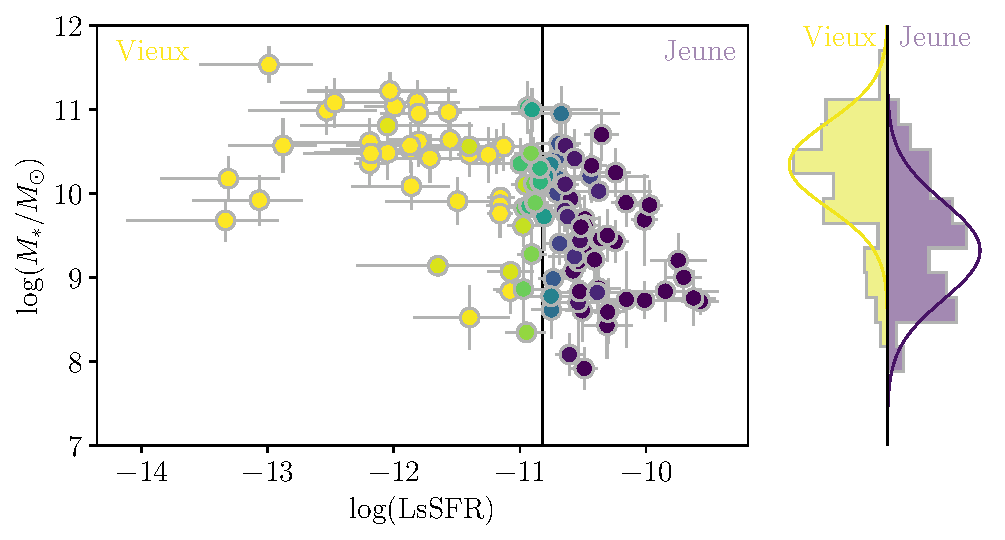
\includegraphics[width=\linewidth]{model_mass_Howell_hist_SED-nonan.pdf}
    \caption[$M_*$ en fonction du LsSFR des SNe~Ia de SNfactory et modèle de
    masse sélectionné ajusté]{\textit{Principal}~: masses des galaxies hôtes
        ($M_*$) ajustées par SED en fonction du LsSFR pour les SNe de SNfactory.
        La couleur correspond à la probabilité $p_y$ que la SN~Ia soit jeune,
        c'est-à-dire qu'elle ait $\log \mathrm{LsSFR} \geq -10,82$
        \citep[voir][et Chapitre~\ref{ch:stretch}]{rigault2020}. \textit{À
        droite}~: histogramme pondéré par $p_y$ des étirements des SNe, ainsi
        que le modèle sélectionné ajusté~; les contributions des populations
    jeune et âgée sont indiquées en violet et jaune, respectivement.}
    \label{fig:massmodel}
\end{figure}

D'après la forme des histogrammes de la Figure~\ref{fig:massmodel}, nous avons
implémentés différentes modélisations. Cette étude étant annexe à la simulation
par \snana, nous ne présentons que les plus pertinentes et omettons les
modélisations n'ayant pas d'intérêt physique ou mathématique, c'est-à-dire les
modélisations constantes avec le redshift (notamment les Gaussienne simple et
Gaussienne asymétrique pure) et les modèles ne convergeant pas. Ainsi, nous
présentons les modèles suivants~:

\begin{itemize}
    \item «~Howell~» d'après~\cite{howell2007}, avec une Gaussienne simple pour
        chacune des populations jeune et âgée (voir Chapitre~\ref{ch:stretch})~;

    \item «~Howell+asym~» où la population jeune est une simple Gaussienne et la
        population vieille est une Gaussienne asymétrique~;

    \item «~Howell asym~» où les deux populations jeune et âgée sont
        asymétriques.
\end{itemize}

\subsection{Comparaison aux données}\label{ssec:mres}

Chacun de ces modèles a été ajusté aux différents échantillons, et nous en
présentons maintenant les résultats. La procédure d'ajustement est celle de la
Section 3 de~\citetalias{nicolas2021}, selon la présence de LsSFR dans chaque
sous-échantillon. On définit de même que précédemment
\begin{equation}\label{eq:likelihood}
    -2\ln(L) = -2 \sum_i \ln \prob{x_1^i}{\vec{\theta};
    \mathrm{d}x_1^i, y^i}.
\end{equation}
et nous utilisons le critère d'information
d'\textsc{Akaike}~\citep[AIC,][]{burnham2004} pour comparer la capacité de
chaque modèle à décrire correctement les données en pénalisant l'ajout de
paramètres libres tel que~:
\begin{equation}
    \mathrm{AIC} = -2\ln(L) + 2k,
\end{equation}
ce qui permet d'éviter le sur-ajustement. Les résultats sont présentés
Tableau~\ref{tab:modelcomp}.

\begin{table}[h]
    \centerfloat
    \begin{threeparttable}
        \caption[Comparaison de la capacité relative de chaque modèle à décrire
        les données selon l'échantillon d'ajustement]{Comparaison de la
            capacité relative de chaque modèle à décrire les données selon
        l'échantillon d'ajustement.}
        \label{tab:modelcomp}
        \begin{tabular}{lcccccccccc}
            %\hline\hline & & & & & & \\[-0.6em]
            \toprule &
            & \multicolumn{3}{c}{Howell ($k=4$)}
            & \multicolumn{3}{c}{Howell+asym ($k=5$)}
            & \multicolumn{3}{c}{Howell asym ($k=6$)} \\
            \cmidrule(lr){3-5}\cmidrule(lr){6-8}\cmidrule(lr){9-11}
            Échantillon & N$_{\rm SNe~Ia}$ &
            $-2\ln(L)$ & AIC & $\Delta$AIC &
            $-2\ln(L)$ & AIC & $\Delta$AIC &
            $-2\ln(L)$ & AIC & $\Delta$AIC\\[0.2em]
            %\hline & & & & & & \\[-0.6em]
            \midrule
            SNf & 114 &
            230,0 & 238,0 & -- &
            229,8 & 239,8 & -1,8 &
            229,7 & 241,7 & -3,7 \\
            SEDSNf & 110 &
            223,9 & 231,9 & -- &
            221,4 & 231,4 & 0,6 &
            221,3 & 233,3 & -1,4 \\
            Fiduciel & 544 &
            1534,3 & 1542,3 & -- &
            1534,3 & 1544,3 & -2,0 &
            1531,0 & 1543,0 & -0,7 \\
            SED Fiduciel & 548 &
            1546,6 & 1554,6 & -- &
            1546,5 & 1556,5 & -1,9 &
            1538,7 & 1550,7 & 4,0 \\
            \bottomrule
        \end{tabular}
        \begin{tablenotes}[flushleft]
            \item\small \textbf{\hspace{-3.2pt}Notes.} Pour chaque modèle
                considéré, nous indiquons son nombre
                de paramètres libres $k$, et pour chaque échantillon étudié son
                $-2\ln(L)$ (voir Équation~\ref{eq:likelihood}), son AIC et la
                différence d'AIC ($\Delta$AIC) entre ce modèle et le modèle
                Howell, choisi comme référence car présentant l'AIC le plus
                faible pour 6 comparaisons sur 8.
        \end{tablenotes}
    \end{threeparttable}
\end{table}

Après calcul, le modèle Howell est celui qui se détache le plus, étant celui de
plus petit AIC pour 6 modèles sur 8, et est celui représenté sur la
Figure~\ref{fig:massmodel}~; cependant tous les modèles sont considérés comme
étant de bonnes représentations des données. Nous présentons
Figure~\ref{fig:mod_comp} une illustration des résultats du tableau précédent,
et Figure~\ref{fig:mod_all} les représentations graphiques des modèles
implémentés variant en redshift.

\begin{figure}[ht]
    \centering
    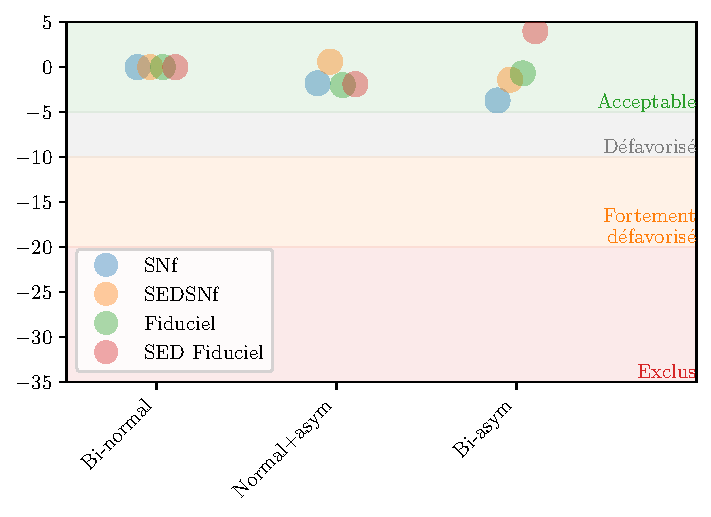
\includegraphics[width=.6\linewidth]{mass_comp_df-nobug}
    \caption[$\Delta$AIC entre le modèle Howell et les autres
    modèles]{$\Delta$AIC entre le modèle Howell et les autres modèles (voir
        Tableau~\ref{tab:modelcomp}). Tous les modèles sont dérivants. Les
        marqueurs bleus, orange, verts, rouges montrent les résultats lorsque
        l'analyse est effectuée sur l'échantillon SNf, SEDSNf, fiduciel,
        fiduciel avec SEDSNf, respectivement (voir légende). Les bandes de
        couleur illustrent la validité des modèles, d'acceptable ($\Delta$AIC >
        -5) à exclu ($\Delta$AIC < -20). En suivant ces valeurs d'AIC, tous les
        modèles sont compatibles entre eux.}
    \label{fig:mod_comp}
\end{figure}

\begin{figure}[htbp]
    \vspace*{-3cm}
    \centerfloat
    \includegraphics[width=1.1\linewidth]{mass_model_all_evol.pdf}
    \caption[Modèles implémentés et testés dans l'étude de l'évolution de
    l'étirement avec le redshift]{\scriptsize Modèles implémentés et testés dans
        l'étude de l'évolution de la masse avec le redshift. Les modèles Howell,
        Howell+asym et Howell asym sont tracés dans la colonne de gauche, du
        milieu et de droite, respectivement. Les échantillons sur lesquels ils
        sont ajustés correspondent aux lignes et à la couleur de fond du
        graphique~: SNf (bleu), SEDSNf (orange), fiduciel (vert), fiduciel avec
        SEDSNf (rouge)~; ce sont les mêmes couleurs que dans la
        Figure~\ref{fig:mod_comp}. Les quantités $\Delta(-2\ln(L))$ et
        $\Delta$AIC par rapport au modèle Howell de chaque ligne sont indiqués
        pour chaque modèle figure. Nous avons tracé dix réalisations des modèles
        selon la valeur du redshift moyen considéré, de la valeur la plus basse
        de notre échantillon ($z = 0,02$) à la valeur maximale des données
        totales (sans coupe en redshift) de SNLS ($z = 1,06$) représentés en
        couleur allant du jaune (bas redshift, plus vieil environnement) au
        violet (haut redshift, environnement jeune) et les distributions des
        populations jeune et vieille constituant le modèle total sont en gris
        pointillé et fin pointillé, respectivement. Nous y retrouvons
        l'information que tous les modèles sont compatibles en tant que bonnes
    représentations des données par rapport au modèle de base.}
    \label{fig:mod_all}
\end{figure}

\subsection{Sélection des modèles}\label{ssec:mmodsel}

Avec la multitude de modèles possibles pour établir nos \hostlib, nous avons dû
effectuer une sélection. Étant donné que notre but est d'associer de manière
cohérente un âge de SN définie par un redshift et une masse de galaxie hôte, une
caractéristique primordiale au modèle choisi est d'avoir une évolution de la
fraction de jeunes SNe~Ia physiquement cohérente avec les observations~; nous
nous attendons notamment à ce que la fraction de jeunes étoiles soit $\approx$ 1
pour les $M_* \gtrsim 10^7\si{\Msun}$, diminue progressivement jusqu'à $\approx
50\%$ pour $M_* \approx 10^{10}\si{\Msun}$ et continue sa progression vers 0
pour $M_* > 10^{10}\si{\Msun}$~; en effet, la position de la marche de magnitude
basée sur la masse est à $M_* = 10^{10}\si{\Msun}$ et cette limite constitue un
bon indicateur de l'âge d'une SN~Ia d'après~\cite{briday2022}.

Nous avons étudié cette évolution pour les différents modèles implémentés, dont
les résultats sont présentés Figure~\ref{fig:ypc}.

\begin{figure}[ht]
    \centerfloat
    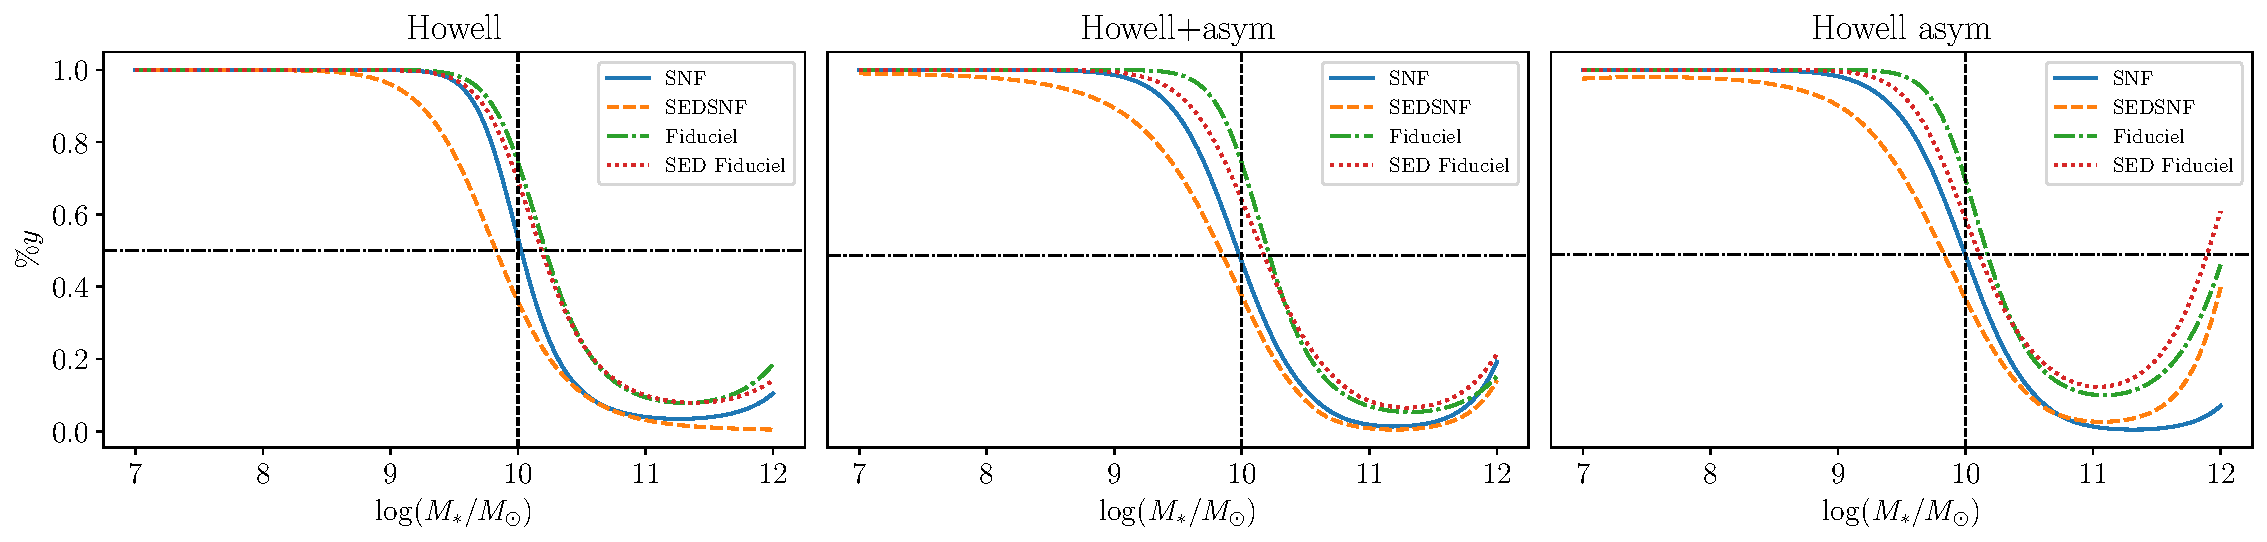
\includegraphics[width=1.2\linewidth]{model_mass_yfrac-best}
    \caption[Comparaison de la prédiction de l'évolution de la fraction de
    jeunes SNe~Ia en fonction de la masse de la galaxie hôte]{Comparaison de la
        prédiction de l'évolution de la fraction de jeunes SNe~Ia ($\%y$) en
        fonction de la masse de la galaxie hôte ($M_*$) pour chaque modèle et
        selon chaque échantillon utilisé pour l'ajustement. Alors que le sens de
        variation devrait être constant, pratiquement tous les modèles finissent
        par remonter après $M_* \approx 10^{11}\si{\Msun}$, sauf le modèle
        Howell ajusté sur SEDSNf. Nous excluons les modèles Howell+asym et
    Howell asym par ce critère.}
    \label{fig:ypc}
\end{figure}

Nous trouvons alors que tous les modèles finissent par présenter une remontée de
la fraction de jeunes étoiles quand la masse $M_* > 10^{11}\si{\Msun}$, sauf le
modèle Howell ajusté sur l'échantillon SEDSNf. Cela provient de l'incertitude
des courbes Gaussiennes des sous-populations jeunes étant bien plus larges que
celles des sous-populations vieilles, donnant pour les masses élevée un rapport
de probabilité en faveur des jeunes SNe~Ia. Ceci ne correspondant pas à une
réalité physique, nous rejetons tous les modèles Howell+asym et Howell asym de
notre étude à partir de ces résultats. Parmi les modèles Howell, seul celui
ajusté sur SNf passe en effet par 50\% à $M_*=10^{10}\si{\Msun}$.

Nous conservons ainsi les modèles suivants~:
\begin{enumerate}
    \item Le modèle Howell ajusté sur SEDSNf~;
    \item Le modèle Howell ajusté sur SNf~;
\end{enumerate}
et pour reproduire artificiellement la descente de la fraction de jeunes étoiles
en fonction de la masse attendue, nous avons également~:
\begin{enumerate}[resume]
    \item «~SNfsupp~» («~suppressed~», «~réprimé~»)~: le modèle Howell ajusté
        sur SNf, mais pour lequel les objets de $M_* > 10^{11}\si{\Msun}$ sont
        automatiquement associés à des SNe~Ia âgées.
\end{enumerate}

Nous prenons le modèle SNfsupp comme référence~; les implications du choix de
modélisation de masse est discuté Section~\ref{sec:modsys}. Les valeurs des
paramètres des modèles SEDSNf et SNf sont indiquées
Tableau~\ref{tab:modelresults}.

\begin{table}[ht]
    \centerfloat
    \caption[Valeurs des paramètres issus des meilleurs ajustement du modèle
    Howell sur les échantillons SNf et SEDSNf]{Valeurs des paramètres issus des
    meilleurs ajustement du modèle Howell sur les échantillons SNf et SEDSNf.}
    \label{tab:modelresults}
    \begin{tabular}{lcccc}
        \toprule
        Échantillon              &
                $\mu_{\rm y} $   &
                $\sigma_{\rm y}$ &
                $\mu_{\rm o} $   &
                $\sigma_{\rm o}$ \\
        \midrule
        SNf    & $9.36  \pm 0.06$
               & $0.64  \pm 0.04$
               & $10.58 \pm 0.04$
               & $0.38  \pm 0.04$
               \\
        SEDSNf & $9.32  \pm 0.07$
               & $0.58  \pm 0.05$
               & $10.34 \pm 0.07$
               & $0.51  \pm 0.06$
               \\
        \bottomrule
    \end{tabular}
\end{table}

\subsection{Génération des \hostlib}\label{ssec:inpgen}

Avec les modélisations de la masse et de l'étirement en fonction du redshift,
nous pouvons à présent lire les entrées des \hostlib\ BP, et à partir d'un
redshift générer une liste de masses et d'étirements. Cela nous permettra
ensuite de faire correspondre la masse de la \hostlib\ avec celles de la liste
générée, et d'attribuer une valeur d'étirement qui remplacera celle
de~\citetalias{popovic2021a}.

Cette étape est réalisée avec le module Python
\texttt{SNprop}\footnote{\label{fn:snprop}\href{
    https://github.com/MickaelRigault/snprop}
{https://github.com/MickaelRigault/snprop}}. Ce processus prend la fraction
attendue de jeunes étoiles en utilisant $\delta(z)$ donnée
Équation~\ref{eq:deltaz}. Il assigne une qualité «~jeune~» (LsSFR = 1) ou
«~vieille~» (LsSFR = 0) au tirage qui va suivre en prenant un nombre aléatoire
$r$ entre 0 et 1 et en le comparant à la valeur de la fraction susmentionnée. Si
$r < \delta(z)$, alors la SN simulée sera jeune et inversement. Plus $z$
augmente et plus $\delta(z)$ augmente, et donc plus la probabilité d'être
assigné jeune augmente. Ceci est présenté Figure~\ref{fig:deltaz}.

\begin{figure}[]
    \centering
    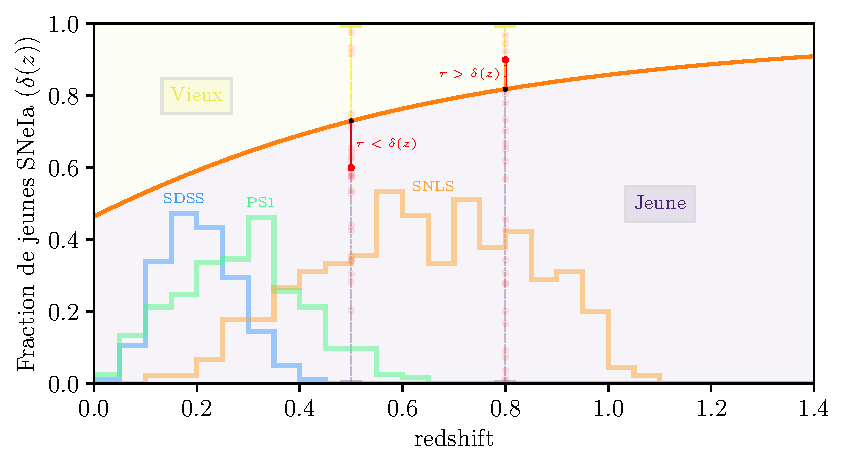
\includegraphics[width=.8\linewidth]{deltaz_hist_yo-random.pdf}
    \caption[Représentation du choix de l'âge d'une SN et de l'assignation de
    masse et d'étirement en fonction du redshift]{Représentation du choix de
        l'âge d'une SN et de l'assignation de masse et d'étirement en fonction
        du redshift du module Python \texttt{SNprop}\footnoteref{fn:snprop}.
        \textit{Orange}~: fraction estimée de jeunes SNe~Ia en fonction du
        redshift. \textit{Histogrammes}~: nombres de SNe~Ia des 3 sondages
        principaux de l'échantillon Pantheon \citep{scolnic2018} (pas à
        l'échelle). \textit{Lignes rouges verticales}~: pour chaque $z$ de la
        \hostlib, un nombre aléatoire $r$ entre 0 et 1 est tiré~: s'il est
        supérieur (inférieur) à $\delta(z)$ à ce redshift, alors la SN sera
        assignée vieille (jeune) et les valeurs de masse et d'étirement générées
        seront tirées des distributions sous-jacentes vieilles (jeunes) des
    paramètres correspondants.}
    \label{fig:deltaz}
\end{figure}

Cette étape est réalisée \num{1000} fois pour chaque redshift de la \hostlib,
donnant une table de redshift, âge (0 ou 1), masse et étirement de \num{1000}
entrées, puis une correspondance est effectuée entre toutes les masses tirées et
la masse de la \hostlib\ pour trouver celle qui en est la plus proche. Nous
prenons alors la valeur d'étirement associée et remplaçons celle de la \hostlib.
Au même moment, nous entrons la valeur de l'âge (0 ou 1) dans une nouvelle
colonne~; ceci conclut la confection des \hostlib\ NN.

Les \hostlib\ NR possèdent un autre colonne supplémentaire, où à chaque valeur
d'âge est associée une valeur de variation de magnitude, de +\SI{0,065}{mag}
pour les jeunes (moins lumineuses) et de -\SI{0,065}{mag} pour les vieilles
(plus lumineuses), qui remplacent le valeurs de marche de magnitude basées sur
la masse implémentées dans les autres approches et qui sont associées au
\wgtmap.

\subsection{Implémentation}\label{ssec:snaimpl} 

Nous pouvons implémenter différentes manières d'effectuer ces simulations, que
nous appelons «~types~». Une approche serait de simuler 100 fois des
échantillons de la taille de l'échantillon de Pantheon ($\approx \num{1000}$) et
de combiner les résultats, permettant ainsi d'avoir des incertitudes
statistiques réalistes. Bien que nous ayons entamé la réalisation d'une telle
approche, le plus simple et moins coûteux en temps a été de simuler un
échantillon d'une taille conséquente ($\approx \num{13 000}$) avec un BiasCor 50
fois plus grand, donnant une idée de l'incertitude systématique due aux
différents modèles de corrélations (SK, BP, NN, NR).

Pour quantifier cela, nous conservons les données simulées et les échantillons
BiasCor associés de chaque modélisation, afin d'utiliser les données d'un modèle
et de les corriger avec le BiasCor d'un autre~: l'idée derrière cette pratique
est de connaître le potentiel biais dû au fait de méconnaître la physique réelle
qui régit les propriétés intrinsèques des SNe~Ia. Pour les distinguer, nous les
nommons de la manière suivante~:
\begin{center}
    \begin{tikzpicture}[]
        \node[anchor=center] (name) at (0,0)
            {\textcolor{cornflowerblue}{SK}\_\textcolor{limegreen}{NR}};
        \node[inner sep=0] (datab) at ([shift={(0,3pt)}]name.south west) {};
        \node[inner sep=0] (biasb) at ([shift={(0,3pt)}]name.south east) {};
        \node[below left =of datab, color=cornflowerblue] (data)
            {Données};
        \node[below right=of biasb, color=limegreen] (bias)
            {BiasCor};
        \draw[-stealth] (data) -- (datab);
        \draw[-stealth] (bias) -- (biasb);
    \end{tikzpicture}
\end{center}
Ainsi, «~SK\_NR~» décrit un échantillon dont les données ont été générées en
supposant les modèles de corrélations de~\citetalias{scolnic2016} et corrigées
avec des données générées en supposant les modèles de corrélations dus à l'âge
(NR). Lorsque les données et BiasCor sont les mêmes, nous ne mentionnons pas
quel est le BiasCor. 

Pour comparer de manière cohérente les données simulées aux données réelles, il
faut que le ratio des données de chaque sondage de l'échantillon simulé
corresponde au ratio des données de chaque sondage de l'échantillon réel. Ceci
s'effectue \textit{via} un paramètre appelé \texttt{NGEN}, décrivant le nombre
d'années de sondage simulé. Il permet de contrôler plus ou moins précisément le
nombre de SNe~Ia simulées, puisque chaque sondage a sa propre efficacité
spectroscopique qui, à chaque simulation, opère une sélection des données
conservées (voir Chapitre~\ref{ch:snana}). Notamment, puisque l'efficacité
spectroscopique de l'échantillon LOWZ est particulièrement faible, il nécessite
un grand \texttt{NGEN} dans nos fichiers de configurations. De plus, la
correction par \bbc\ réduit l'échantillon en ne conservant que les données qui
sont dans un intervalle de BiasCor avec suffisamment de points pour avoir une
valeur de correction. Nous indiquons dans le Tableau~\ref{tab:ratio} le
nombre de données pour les données réelles et pour nos simulations, exprimées en
pourcentages de l'échantillon Pantheon.

\begin{table}[ht]
    \centerfloat
    \begin{threeparttable}
        \caption[Nombre de données de nos différentes simulations]{Nombre de
            données après l'ajustement par \bbc\ et après
            l'échantillonnage nécessaire à la reproduction des ratio
        observés dans l'échantillon Pantheon \citep{scolnic2018}.}
        \label{tab:ratio}
        \begin{tabular}{ccccccc}
            \toprule & &
            \multicolumn{5}{c}{Après \bbc} \\
            \cmidrule(lr){3-7}
            Données & BiasCor &
            Total (\%) & LOWZ & SDSS & PS1 & SNLS \\
            \midrule
            \multicolumn{2}{c}{Pantheon} &
            1022 & 172 & 335 & 279 & 236 \\
            \midrule
            \multirow{4}{*}{SK} 
            & SK & 13333 (13.05) & 13.64 & 7.29 & 19.63 & 13.00 \\
            & BP & 12847 (12.57) & 13.31 & 7.00 & 19.24 & 12.06 \\
            & NN & 12898 (12.62) & 13.03 & 7.01 & 19.40 & 12.27 \\
            & NR & 12898 (12.62) & 13.03 & 7.01 & 19.40 & 12.27 \\
            \midrule
            \multirow{4}{*}{BP}
            & SK & 12316 (12.05) & 10.50 & 6.71 & 18.10 & 13.61 \\
            & BP & 12462 (12.19) & 10.59 & 6.77 & 18.66 & 13.42 \\
            & NN & 12397 (12.13) & 10.02 & 6.76 & 18.68 & 13.55 \\
            & NR & 12397 (12.13) & 10.02 & 6.76 & 18.68 & 13.55 \\
            \midrule
            \multirow{4}{*}{NN}
            & SK & 12439 (12.17) & 12.59 & 6.54 & 17.87 & 13.12 \\
            & BP & 12478 (12.21) & 12.51 & 6.57 & 18.33 & 12.75 \\
            & NN & 12787 (12.51) & 13.09 & 6.61 & 18.73 & 13.11 \\
            & NR & 12787 (12.51) & 13.09 & 6.61 & 18.73 & 13.11 \\
            \midrule
            \multirow{4}{*}{NR}
            & SK & 12461 (12.19) & 13.01 & 6.60 & 17.89 & 12.81 \\
            & BP & 12475 (12.21) & 12.88 & 6.62 & 18.32 & 12.41 \\
            & NN & 12798 (12.52) & 13.49 & 6.70 & 18.72 & 12.76 \\
            & NR & 12798 (12.52) & 13.49 & 6.70 & 18.72 & 12.76 \\
            \bottomrule
        \end{tabular}
        \begin{tablenotes}[flushleft]
            \item \small \textbf{\hspace{-3,2pt}Notes.} Les pourcentages
                sont indiqués par rapport à la taille de l'échantillon
                Pantheon, voir première ligne. Les sous-échantillons simulés
                sont indiqués en pourcentages directement.
        \end{tablenotes}
    \end{threeparttable}
\end{table}

\appssec{Résumé}{ssec:sumup}

Ainsi, nous avons implémenté dans \snana\ les différentes corrélations
sous-jacentes et modélisations des propriétés des SNe~Ia des études
de~\citetalias{scolnic2016}, \citetalias{popovic2021a}, \citetalias{nicolas2021}
et de cette thèse (NR) \textit{via} le biais de \hostlib. Ces simulations nous
permettent de générer des échantillons corrigés des biais reproduisant les
observations des sondages LOWZ, SDSS, PS1 et SNLS comprenant $\approx
\num{13000}$ données. Ces différentes modélisations peuvent être combinées entre
elles pour tester la qualité des hypothèses sous-jacentes et le possible biais
dû au fait de mal corriger les SNe~Ia. Nous traitons maintenant de la qualité
d'ajustement des données simulées aux données réelles.

\section{Comparaison des données simulées aux données réelles}\label{sec:comp}

Avant de comparer les résultats cosmologiques, nous nous sommes intéressæ à la
correspondance entre les données simulées et les données réelles afin
d'apprécier les implications sur les distributions des différentes
modélisations. Nous présentons dans cette section les différents diagnostiques
nous permettant de comparer à la fois graphiquement et numériquement l'accord
entre les données simulées et données réelles. Pour avoir une comparaison
efficace, nous effectuons une sélection aléatoire des données de chaque sondage
pour reproduire les ratio attendus. Les quantités de données de ces mesures,
exprimées en pourcentages de l'échantillon Pantheon, sont égales aux ratios du
plus petit sondage simulé des données non échantillonnées~: ceux de la colonne
«~SDSS~» du Tableau~\ref{tab:ratio}.

Nous rappelons que les modèles~\citetalias{popovic2021a}
et~\citetalias{scolnic2016} utilisent des distributions des paramètres
spécifiquement ajustés aux données~; BP utilisent des distributions gaussiennes
asymétriques, avec 3 paramètres libres, dans des intervalles de
\SI{0.2e10}{\Msun} (10 pour LOWZ, 20 pour les autres) pour reproduire
l'étirement des SNe~Ia~; SK incluent également des distributions gaussiennes
asymétriques, une pour chacun des sondages SDSS, PS1 et SNLS, et la distribution
donnée Équation~\ref{eq:sklowz} avec 6 paramètres libres, pour un total de $k =
15$. À l'inverse, les modélisations NN et NR reposent sur une modélisation
prospective, basée sur une modélisation de l'étirement avec 5 paramètres libres,
une modélisation de la masse avec 4 paramètres libres, et l'évolution de la
fraction de jeunes étoiles de 2 paramètres libres ($K$, $\Phi$).

Nous nous intéressons dans un premier temps à l'ajustement en 1 dimension des
paramètres (Section~\ref{ssec:comp1d}) avant de traiter l'aspect bi-dimensionnel
(Section~\ref{ssec:comp2d}).

\subsection{Accord entre les données~: analyse uni-dimensionnelle}\label{ssec:comp1d}

Nous présentons ici les résultats des simulations de paramètres de redshift,
étirement et masse des différentes modélisations dont les représentations
graphiques sont données Figure~\ref{fig:hist1d}.

\begin{figure}[ht]
    \centering
    \includegraphics[width=.8\linewidth]{snana_diagnostic_hist_all-panth_only_allSNFSUPP}
    \caption[Histogrammes uni-dimensionnels des données simulées et réelles]
        {Histogrammes normés des données simulées (en lignes pleines
        colorées) et des données réelles (en gris) selon le modèle et le
        paramètre. \textit{De gauche à droite}~: résultats pour les modèles SK,
        BP, NN et NR, respectivement. \textit{De haut en bas}~: nombre de
        données simulées en fonction du redshift, de l'étirement et de la masse,
        respectivement. Les valeurs de $\chi^2$ entre les données simulées et
        réelles sont indiquées dans le coin supérieur droit de chaque figure, et
        de vert à rouge du plus petit au plus grand. Nous indiquons en points
        noirs le modèle d'étirement de~\citetalias{nicolas2021} au redshift
        moyen de l'échantillon Pantheon.}
    \label{fig:hist1d}
\end{figure}

Pour chacune des comparaison, nous calculons une valeur de $\chi^2$. Pour cela,
nous normalisons les histogrammes des données simulées au nombre de données de
Pantheon, puis calculons~:
\begin{equation}\label{eq:chi21d}
    \chi^2 = \frac{1}{N}\times\sum_{i=0}^{N-1} \frac{(d_i - s_i)^2}{d_i+s_i}
\end{equation}
avec $N$ le nombre d'intervalles des histogrammes et $d_i$ ($s_i$) le nombre de
données réelles (simulées) dans l'intervalle $i$. Le meilleur accord est décrit
par le $\chi^2$ le plus petit. Les valeurs sont indiquées
Tableau~\ref{tab:chi21d}.

\newcommand{\ccg}{\cellcolor{limegreen!20}}
\newcommand{\ccr}{\cellcolor{red!10}}
\newcommand{\ccy}{\cellcolor{yellow!20}}
\newcommand{\cco}{\cellcolor{orange!20}}
\begin{table}[ht]
    \centering
    \begin{threeparttable}
        \caption[Comparaison de la capacité de chaque simulation à représenter
        les données en une dimension]{Valeurs de $\chi^2$ donnant la comparaison
            de la capacité de chaque simulation à représenter les données de
        redshift, d'étirement et de masse.}
        \label{tab:chi21d}
        \begin{tabular}{lcccc}
            \toprule
                    & \multicolumn{4}{c}{$\chi^2$} \\ \cmidrule(lr){2-5}
            Paramètre & SK & BP & NN & NR \\
            \midrule
            Redshift    & \ccg\ 4.34  & \ccy\ 4.92  & \cco\ 5.36  & \ccr\ 6.26 \\
            Étirement   & \ccr\ 5.01  & \ccg\ 2.91  & \cco\ 4.01  & \ccy\ 3.83 \\
            Masse       & \ccr\ 4.97  & \cco\ 4.43  & \ccy\ 3.96  & \ccg\ 3.58 \\
            \midrule
            Somme       & \ccr\ 14.32 & \ccg\ 12.26 & \ccy\ 13.33 & \cco\ 13.67\\
            Probabilité & \ccr\ 0.36  & \ccg\ 1.00  & \ccy\ 0.59  & \cco\ 0.49 \\
            \bottomrule
        \end{tabular}
        \begin{tablenotes}[flushleft]
            \item \small \textbf{\hspace{-3,2pt}Notes.} Pour chaque simulation,
                une sélection des données est réalisée pour correspondre aux
                ratios des données de Pantheon, et le calcul du $\chi^2$ est la
                moyenne sur 500 de ces tirages à chaque fois. La probabilité est
                données par rapport au meilleur modèle (BP), telle que
                $\mathcal{P}_{\text{modèle}} =
                \exp^{(\chi^2_{\rm BP} - \chi^2_{\text{modèle}})/2}$.
        \end{tablenotes}
    \end{threeparttable}
\end{table}

D'une manière globale, le modèle BP apparaît comme la meilleure description des
données, NN et NR donnent des résultats similaires et SK a le moins bon accord.
Pour le redshift cependant, c'est le modèle SK qui est le mieux ajusté aux
données~; ceci correspond à nos attentes puisque leurs distributions
d'étirements se divisent par redshift. Pour la masse, étant donné que toutes les
simulations utilisent les mêmes \wgtmap, les différences sont moins notables. NR
donne cependant une meilleure représentation des données, mais pas de manière
significative. Pour l'étirement, c'est BP qui décrit le mieux les données~; ceci
correspond également à nos attentes puisque leurs distributions d'étirement sont
nombreuses. Nous notons cependant que pour ce paramètre, les modèles NN et NR
sont bien représentatifs des données, mais ont par contre une certaine
difficulté à reproduire la distribution de LOWZ. En effet, par la nature ciblée
du sondage, la prédiction du modèle de~\citetalias{nicolas2021} ne peut
s'appliquer, ce qui mène à leurs valeurs de $\chi^2$. Nous présentons
Figure~\ref{fig:lowz1d} l'accord entre données simulées et réelles de
l'échantillon LOWZ pour les différents modèles.

\begin{figure}[ht]
    \centering
    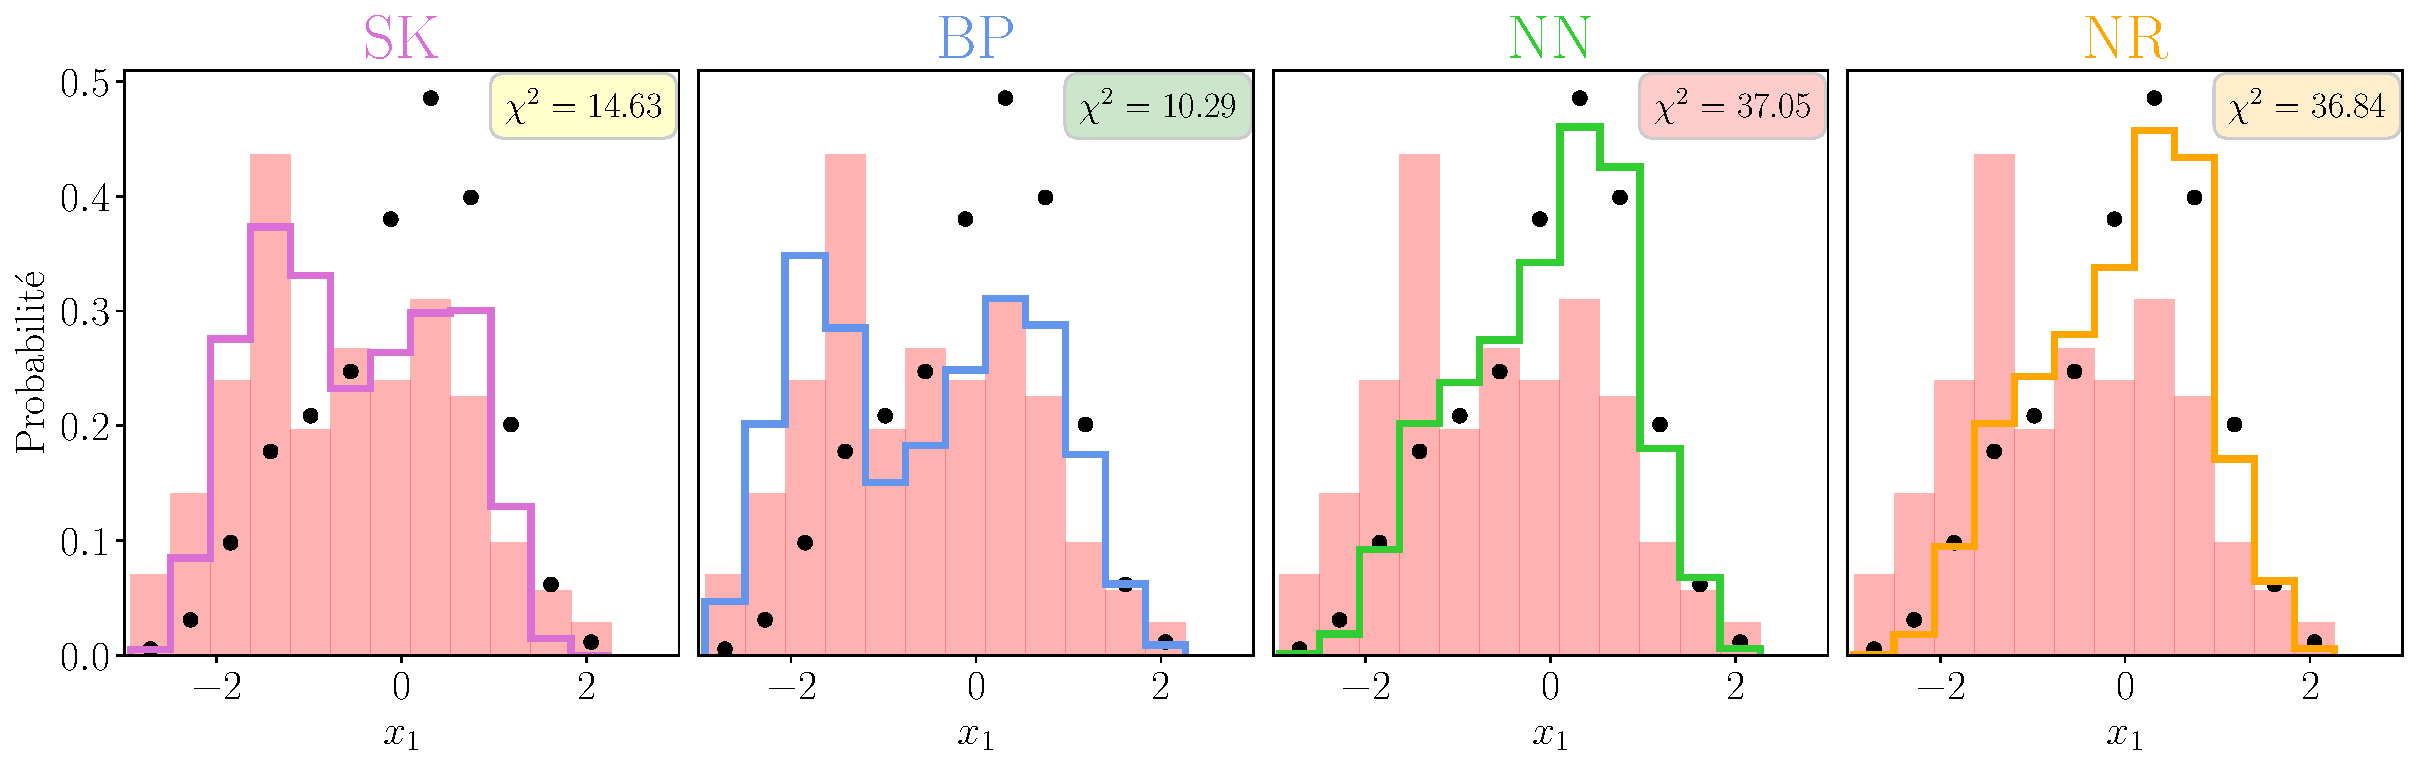
\includegraphics[width=\linewidth]{snana_diagnostic_hist_x1-panth_LOWZ_SNFSUPP}
    \caption[Histogrammes uni-dimensionnels des étirements des données simulées
    et réelles pour l'échantillon LOWZ]{Histogrammes normés des étirements des
        données simulées (en lignes pleines colorées) et des données réelles (en
        rouge) pour le sondage LOWZ selon le modèle. \textit{De gauche à
        droite}~: résultats pour les modèles SK, BP, NN et NR, respectivement.
        Les valeurs de $\chi^2$ entre les données simulées et réelles sont
        indiquées dans le coin supérieur droit de chaque figure, et de vert à
        rouge du plus petit au plus grand. Nous indiquons en points noirs le
        modèle d'étirement de~\citetalias{nicolas2021} au redshift moyen de
    l'échantillon LOWZ.}
    \label{fig:lowz1d}
\end{figure}

Il reste que dans la pratique, tous sondages confondus, les résultats des
différents modèles sont compatibles entre eux, et nous pouvons tous les
considérer comme de bonnes représentations des données. Pour LOWZ
spécifiquement, nous pourrions améliorer la simulation du sondage \textit{via}
la modification du modèle~\citetalias{nicolas2021} pour l'étirement, notamment
en incluant les données de ZTF (Chapitre~\ref{ch:stretch}
Section~\ref{ssec:zres}) ou en utilisant la fraction de jeunes étoiles
escomptée. En effet, le modèle d'évolution de la fraction de jeunes étoiles
$\delta(z)$ donne une valeur de 50\% de jeunes SNe~Ia à $z = 0,05$~; or dans
notre cas, le sondage se situe à un redshift moyen de $z = 0,03$ mais les
données testées (voir Chapitre~\ref{ch:snana}, Figure~\ref{fig:snana_func}) du
modèle NR n'en possèdent que 20\%, réduit à 15\% dans les données conservées.
Comme nous avons créé notre \hostlib\ en utilisant le redshift de chaque entrée,
l'accord avec les données est de fait erroné, et il est probable que la vraie
fraction soit encore plus faible en observant ces résultats
Figure~\ref{fig:lowzdump}.

\sidecaptionvpos{figure}{c}
\begin{SCfigure}[1][ht]
    \centering
    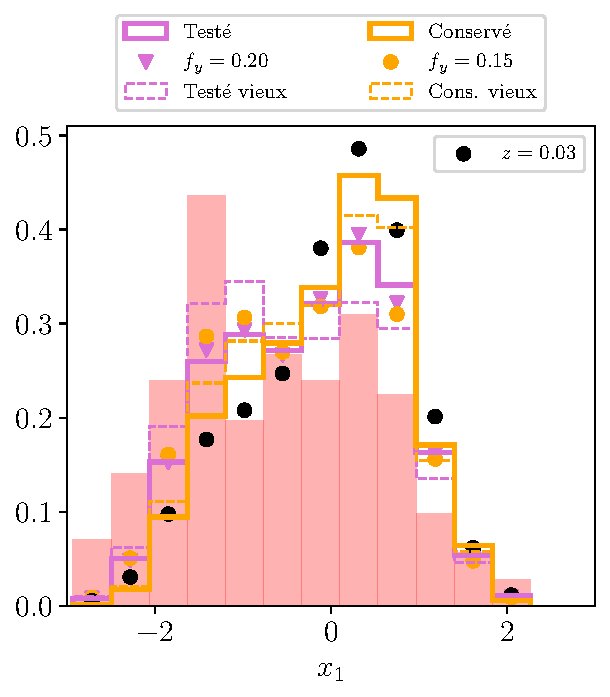
\includegraphics[width=.5\linewidth]{snana_diagnostic_hist_x1-panth_surv_NRSNFSUPP-LOWZ}
    \caption[Histogrammes des données testées et conservées du modèle NR pour le
    sondage LOWZ]{Histogrammes des étirements des données de LOWZ~:\textit{en
        rouge} celles de Pantheon~; \textit{en violet} les données testées et
        \textit{en orange} les données conservées pour le modèle NR. Le
        modèle~\citetalias{nicolas2021} évalué aux fractions des jeunes SNe~Ia
        pour ces deux échantillons sont tracés en marqueurs de la couleur
        correspondante~; le modèle évalué au redshift moyen de la distribution
        est tracé en marqueurs noirs. Les parties vieilles des données testées
    et conservées sont en pointillés.}
    \label{fig:lowzdump}
\end{SCfigure}
\sidecaptionvpos{figure}{t}

\subsection{Accord entre les données~: analyse
bi-dimensionnelle}\label{ssec:comp2d}

Nous présentons maintenant les distributions d'étirement en fonction du redshift
d'une part et les distributions d'étirement en fonction de la masse de la
galaxie hôte d'autre part. Pour déterminer l'accord entre les échantillons réels
et simulés de manière quantitative, nous avons utilisé une estimation par noyau
pour convertir les données simulées en densité de probabilité bi-dimensionnelle,
permettant de calculer une probabilité totale traduisant l'accord entre les
données réelles et le noyau. Deux exemples sont donnés Figure~\ref{fig:2dhex},
où nous représentons les distributions des données simulées \textit{via} son
estimation par noyau en couleurs et en points dispersés pour les données
réelles. Les résultats sont indiqués dans le Tableau~\ref{tab:chi2comp}~: une
plus grande probabilité représente un meilleur accord.

\begin{figure}[ht]
    \centering
    \begin{subfigure}[]{.48\linewidth}
        \centering
        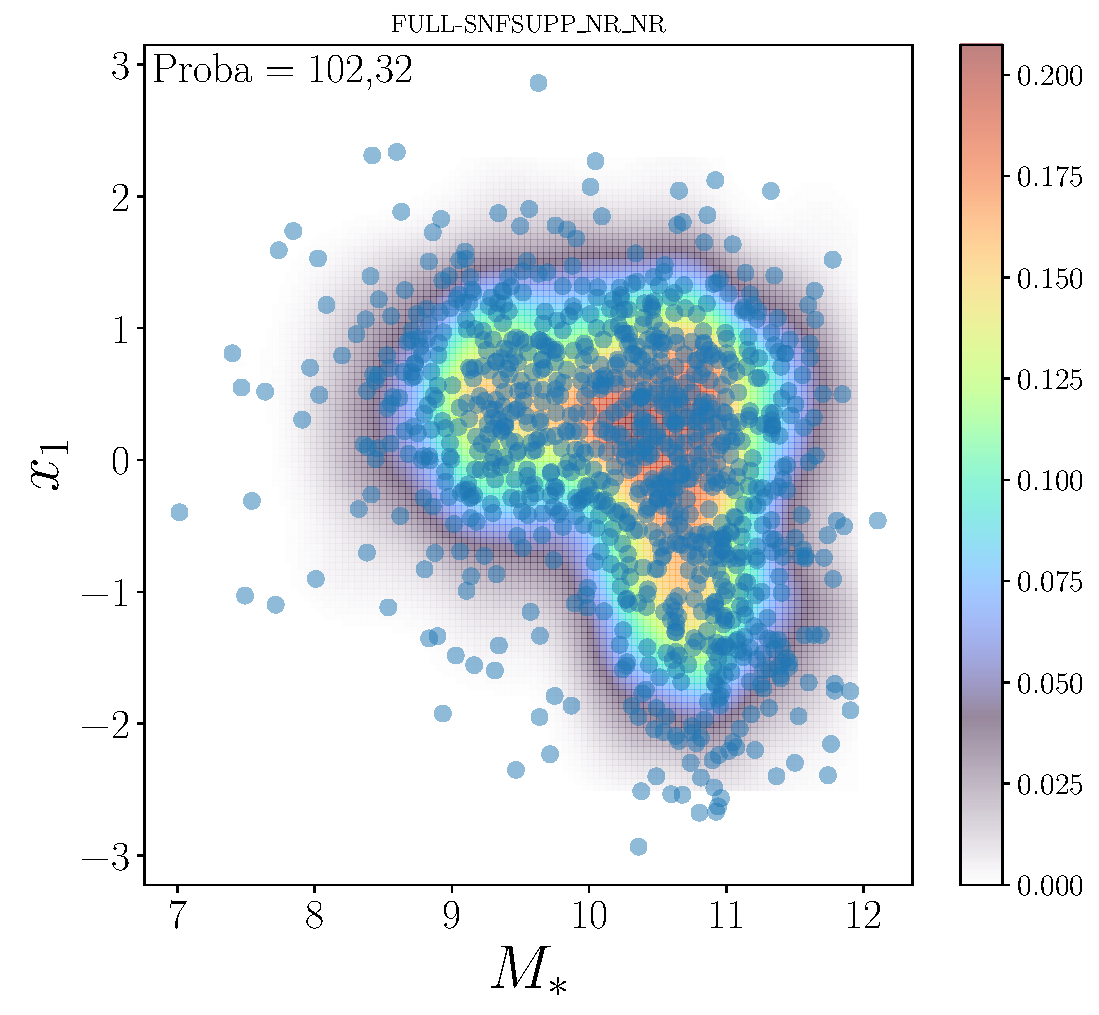
\includegraphics[width=\linewidth]{FULL-SNFSUPP_NR_NR_MS_kernel}
        \caption[Accord entre données réelles et simulées pour les paramètres de
        masse et d'étirement]{\footnotesize\textit{En abscisse}~: masse
        ($> 10^7\si{\Msun}$).\\\hspace*{15.5pt}
        \textit{En ordonnée}~: étirement.}
        \label{fig:hexnrms}
    \end{subfigure}
    \hfill
    \begin{subfigure}[]{.48\linewidth}
        \centering
        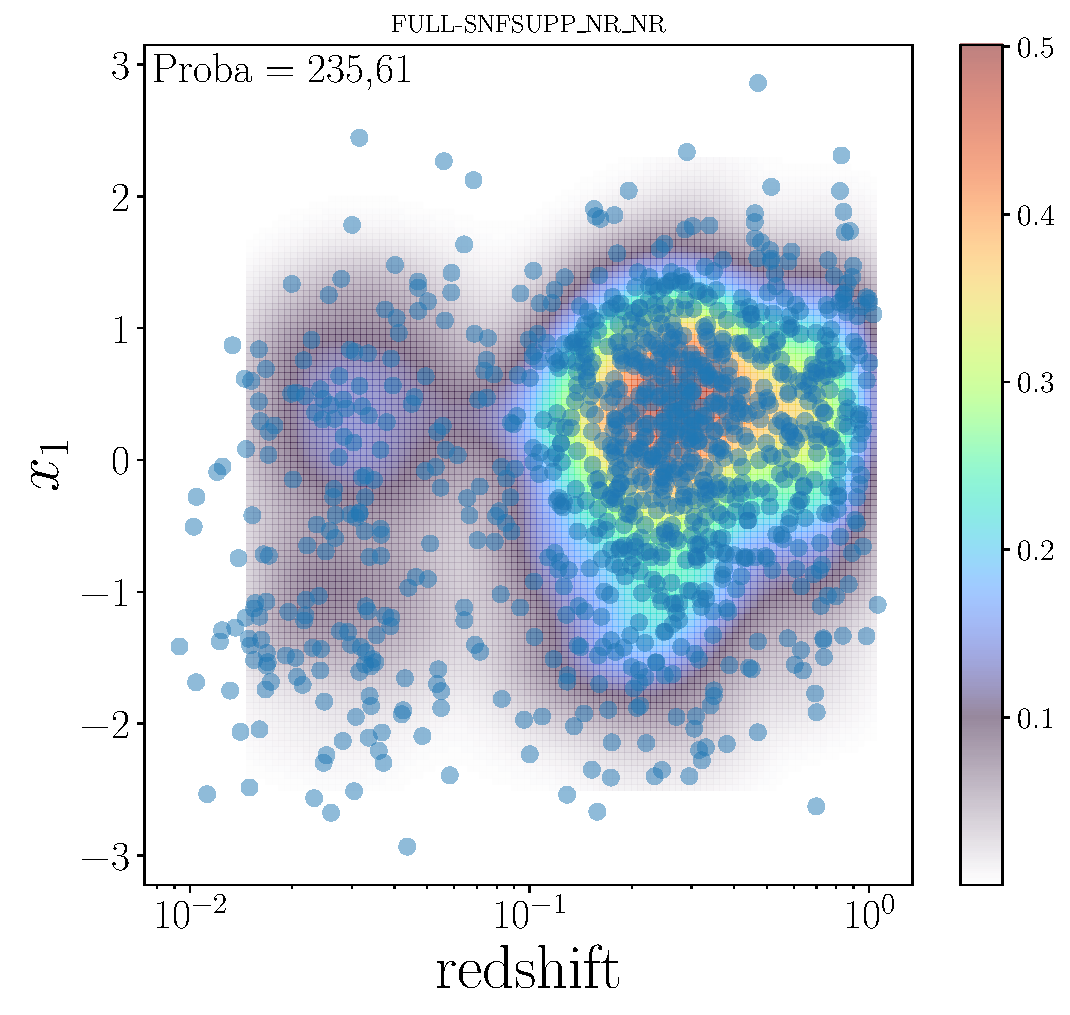
\includegraphics[width=\linewidth]{FULL-SNFSUPP_NR_NR_RS_kernel}
        \caption[Accord entre données réelles et simulées pour les paramètres de
        redshift et d'étirement]{\footnotesize\textit{En abscisse}~: redshift
        (logarithmique).\\\hspace*{15.5pt}
    \textit{En ordonnée}~: étirement.}
        \label{fig:hexnrrs}
    \end{subfigure}
    \caption[Accord entre les données réelles et simulées pour le modèle
    NR]{Accord entre les données réelles et simulées pour le modèle NR.
        L'estimation par noyau donnant la densité de probabilité est indiquée en
        couleur (voir la barre de couleur). L'accord est indiqué sous la forme
    d'une probabilité en haut à gauche.}
    \label{fig:2dhex}
\end{figure}

\begin{table}[ht]
    \centering
    \begin{threeparttable}
        \caption[Comparaison de la capacité de chaque simulation à représenter
        les données en deux dimensions]{Comparaison de la capacité de chaque
            simulation à représenter les données d'étirement et de masse d'une
        part, et d'étirement et de redshift d'autre part.}
    \label{tab:chi2comp}
    \begin{tabular}{lccc}
        \toprule
                & \multicolumn{3}{c}{Probabilité} \\ \cmidrule(lr){2-4}
        Modèles & $x_1$ vs $M_*$ & $x_1$ vs $z$ & Somme \\
        \midrule
        \ccg\ SK & \ccy\ 103,03 & \ccg\ 252,57 & \ccg\ 355,60 \\
        \ccy\ BP & \ccg\ 103,37 & \ccy\ 246,49 & \ccy\ 349,85 \\
        \cco\ NN & \cco\ 102,35 & \cco\ 236,25 & \cco\ 338,60 \\
        \ccr\ NR & \ccr\ 102,32 & \ccr\ 235,61 & \ccr\ 338,93 \\
        \bottomrule
    \end{tabular}
    \begin{tablenotes}[flushleft]
        \item \small \textbf{\hspace{-3,2pt}Notes.} Pour chaque simulation, nous
            calculons une estimation par noyau bi-dimensionnelle sur les données
            simulées et nous l'utilisons pour déterminer chaque probabilité.
    \end{tablenotes}
    \end{threeparttable}
\end{table}

Nous observons que la modélisation~\citetalias{scolnic2016} est la meilleure des
4 sur la combinaison de ces des distributions~; la
modélisation~\citetalias{popovic2021a} est deuxième, et les
modélisations~\citetalias{nicolas2021} et NR on un score similaire les plaçant
comme les modélisations les moins bien ajustées aux données. Les résultats
ne diffèrent que très peu sur les distributions conjointes de redshift et
d'étirement, et la différence

\section{Impact sur la cosmologie~: $w$}\label{sec:simres}

Maintenant que nous avons observé l'accord de chacun de modèles aux données
réelles, nous pouvons étudier le biais cosmologique du fait de traiter des
données ayant leur propre physique avec une correction potentiellement
différente. Pour cela, comme introduit Section~\ref{ssec:snaimpl}, nous
appliquons la méthode BBC7D \citep[][voir Chapitre~\ref{ch:snana}
Section~\ref{ssec:bbc7D}]{popovic2021a} sur les données des différents modèles
avec chacun des échantillons de BiasCor. Nous obtenons ainsi 16 échantillons
corrigés (dont le nombre de données est indiqué Tableau~\ref{tab:ratio}), chacun
ayant une valeur de $w$, $\gamma$, $\alpha$ et $\beta$~; pour rappel, nous avons
fixé $\Omega_M$ à $\num{0.315}\pm\num{0.005}$, et nous ne nous intéressons donc
pas à la variation de ce paramètre.


What we want is not so much $w$ than $\Delta w$ wrt. best current work. We find
x\% and here are the contours.

\begin{figure}[ht]
    \centering
    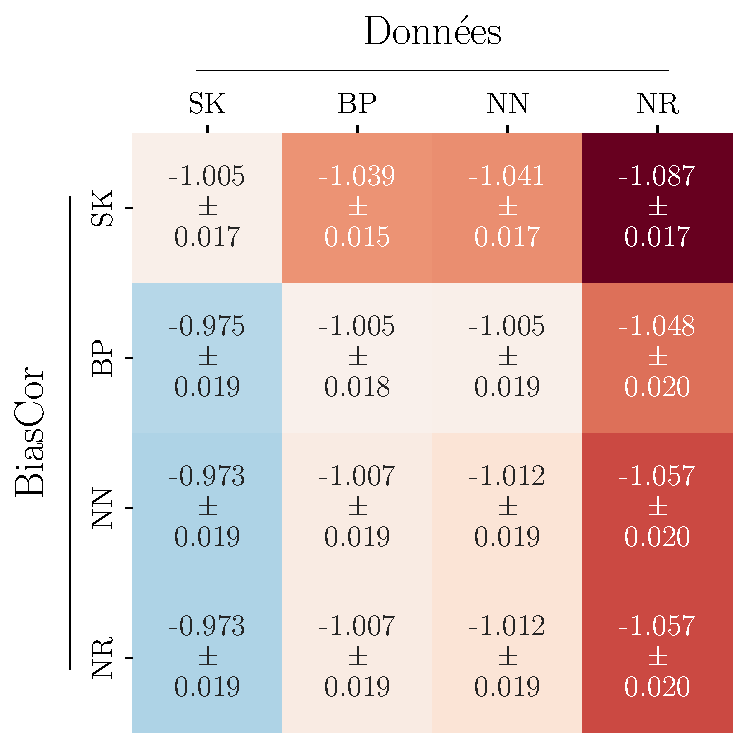
\includegraphics[width=.5\linewidth]{wfit_covmat_FULL-SNFSUPP_2}
    \caption[]{Valeurs de $w$ déterminées par ajustement avec la méthode BBC7D
    \citepalias[][voir Chapitre~\ref{ch:snana}]{popovic2021a}}
    \label{fig:wfit}
\end{figure}

\begin{figure}[ht]
    \centering
    \begin{subfigure}[]{.48\linewidth}
        \centering
        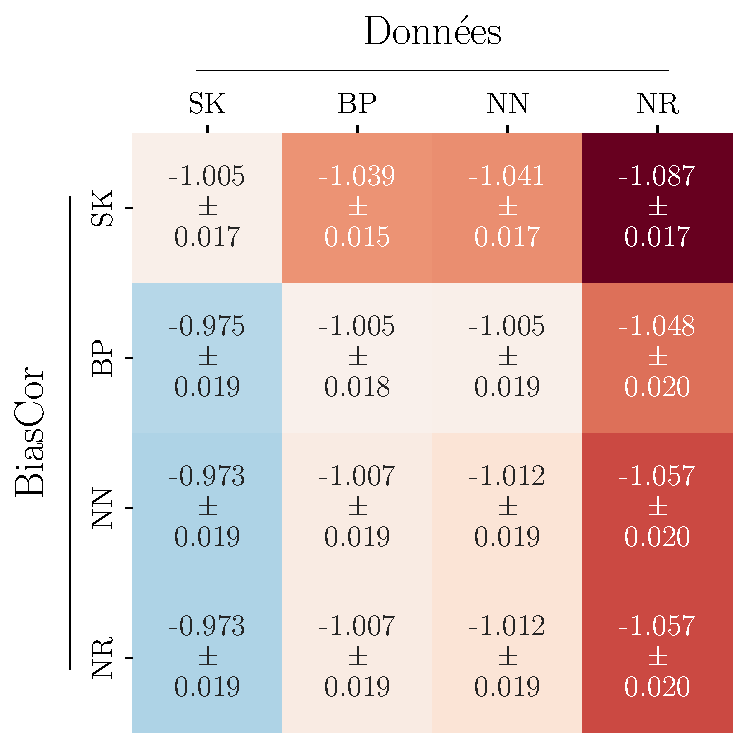
\includegraphics[width=\linewidth]{wfit_covmat_FULL-SNFSUPP_2}
        \caption[Valeurs de $w$ avec le modèle de masse SNfsupp]{Valeurs de
        $w$.}
        \label{fig:cosmow}
    \end{subfigure}
    \hfill
    \begin{subfigure}[]{.48\linewidth}
        \centering
        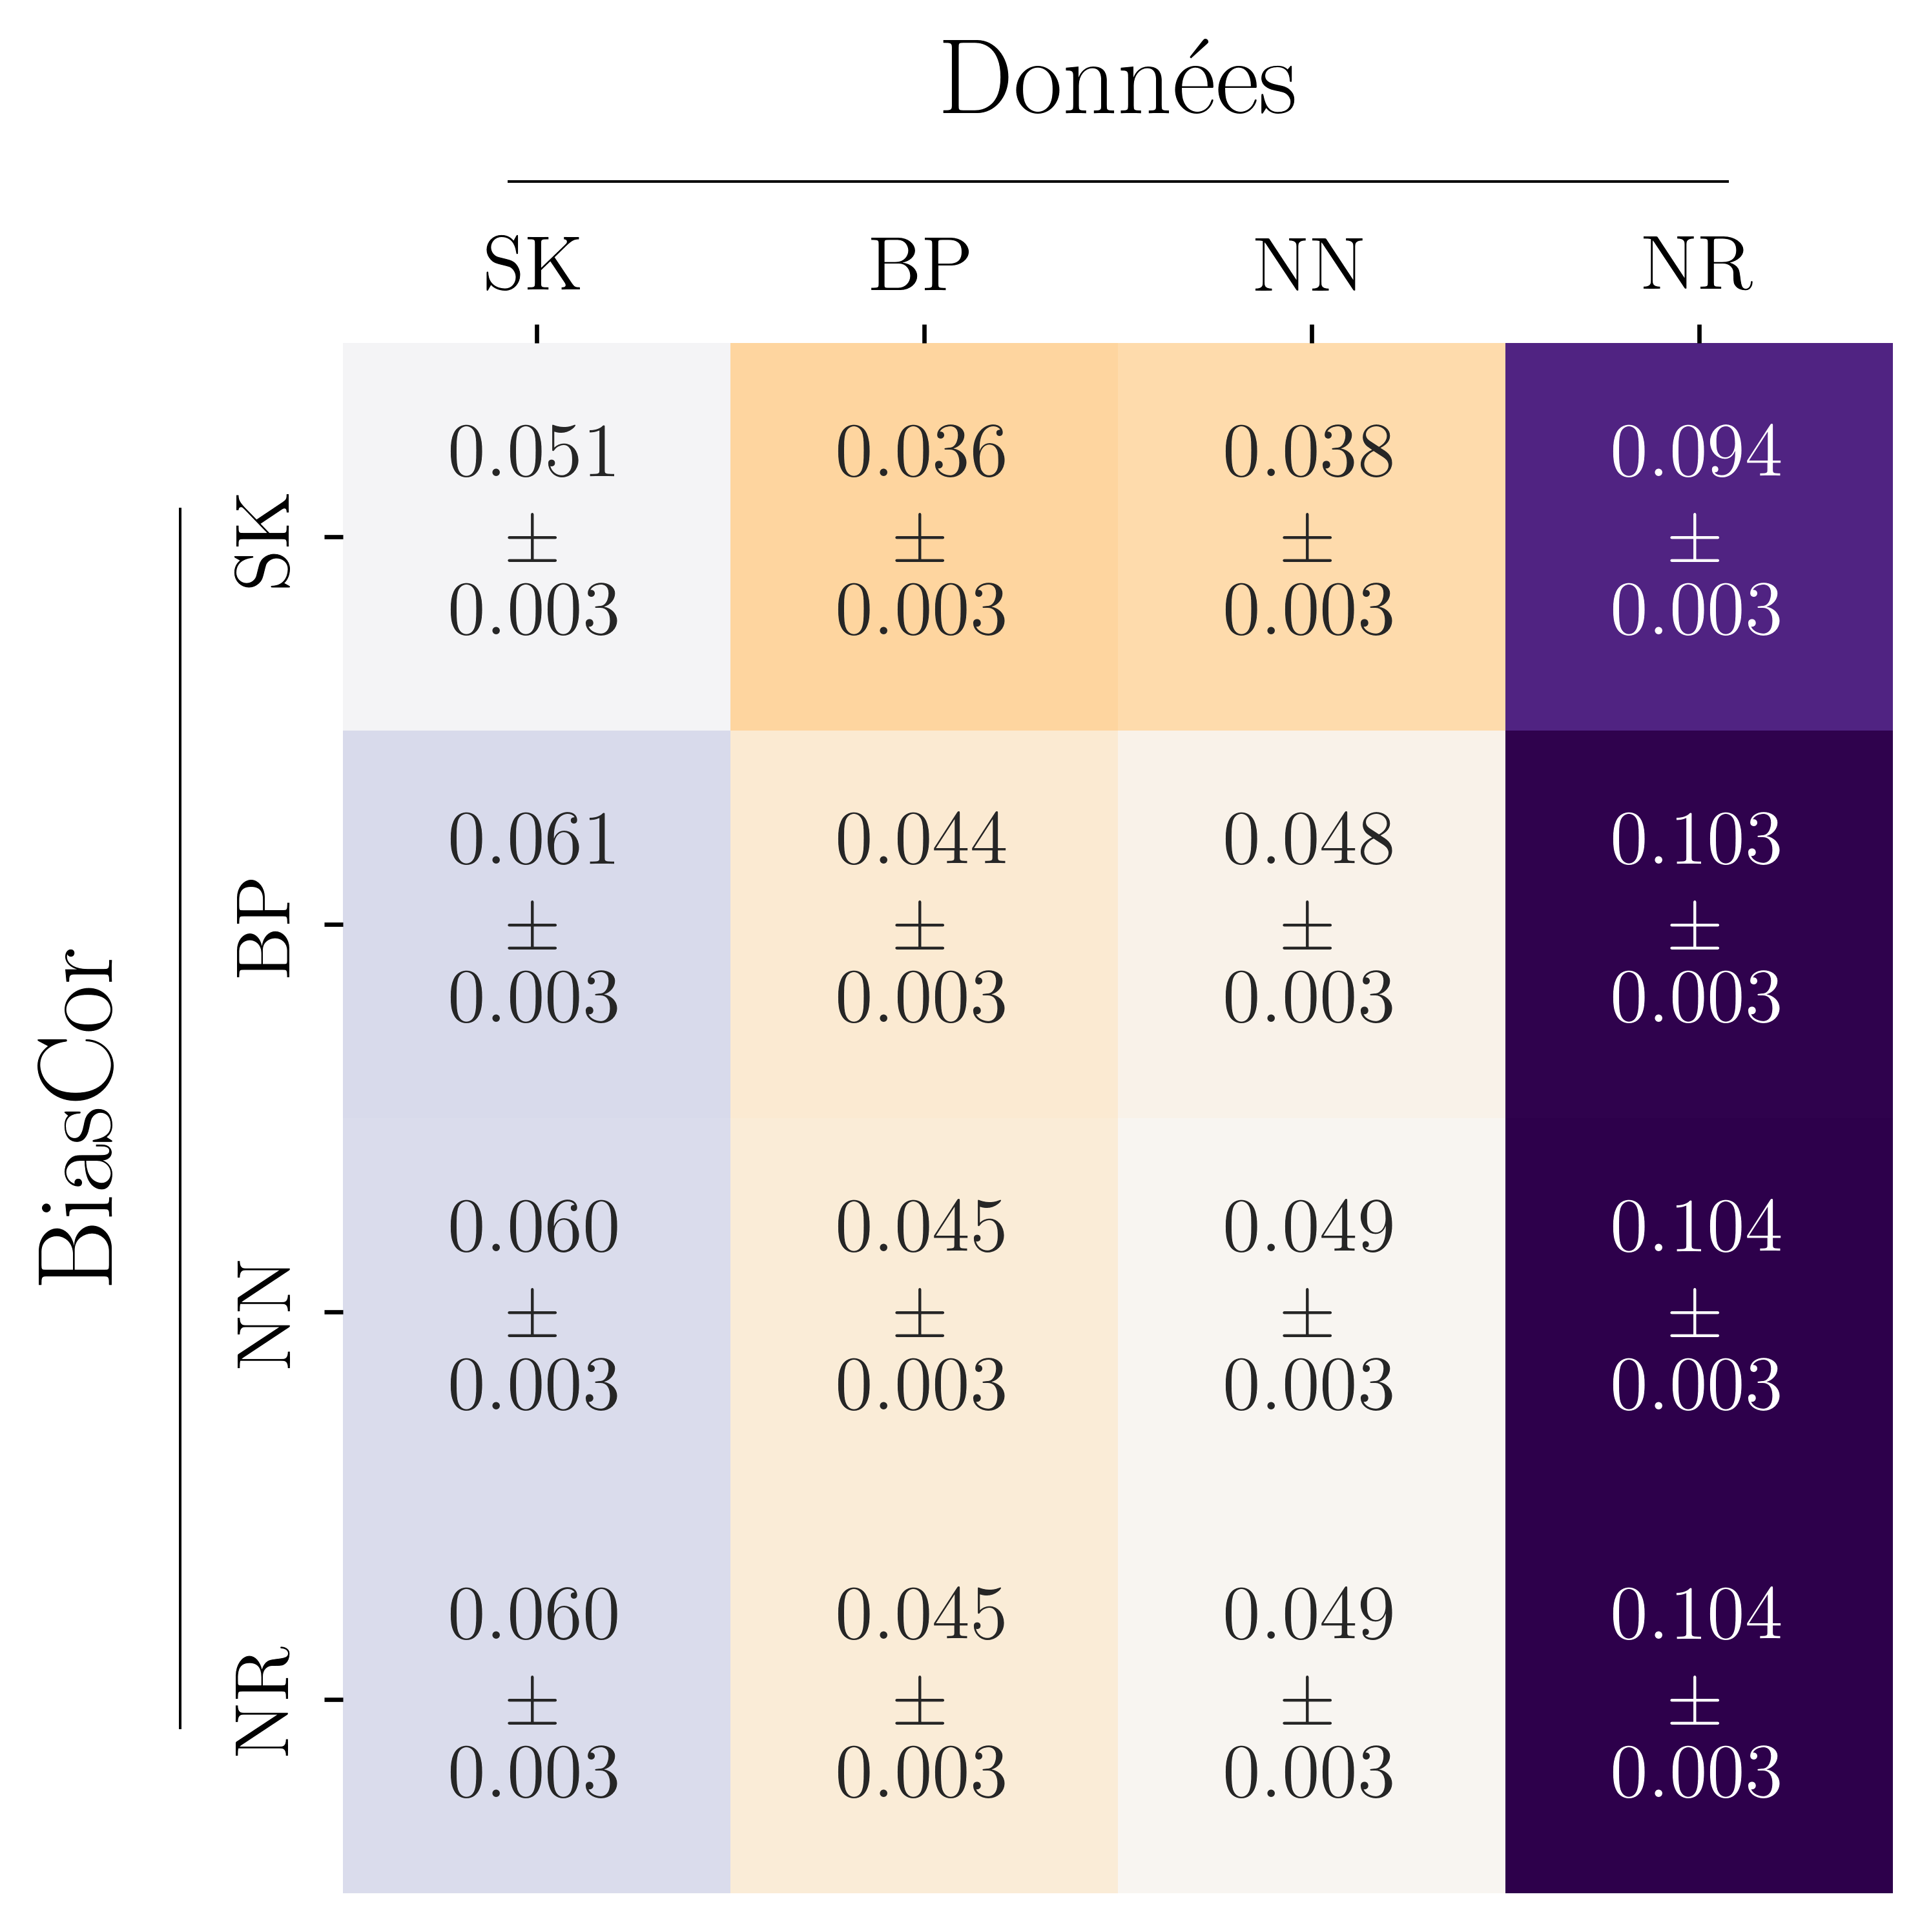
\includegraphics[width=\linewidth]{gammafit_covmat_FULL-SNFSUPP_2}
        \caption[Valeurs de $\gamma$ avec le modèle de masse SNfsupp]{Valeurs de
        $\gamma$.}
        \label{fig:cosmow}
    \end{subfigure}
    \caption[Résultats cosmologiques~: $w$ et $\gamma$]{Résultats
        cosmologiques~: valeurs de $w$ et $\gamma$ déterminées par ajustement
        avec la méthode BBC7D \citepalias[][voir
    Chapitre~\ref{ch:snana}]{popovic2021a}}
    \label{fig:cosmo}
\end{figure}

\section{Discussion}\label{sec:simdisc}
We expected to have a higher/lower, and we got that.

\section{Systématiques dues au choix du modèle de masse}\label{sec:modsys}


\section{Conclusion}\label{sec:simccl}

Should be nice.

\begin{figure}[p]
    \centering
    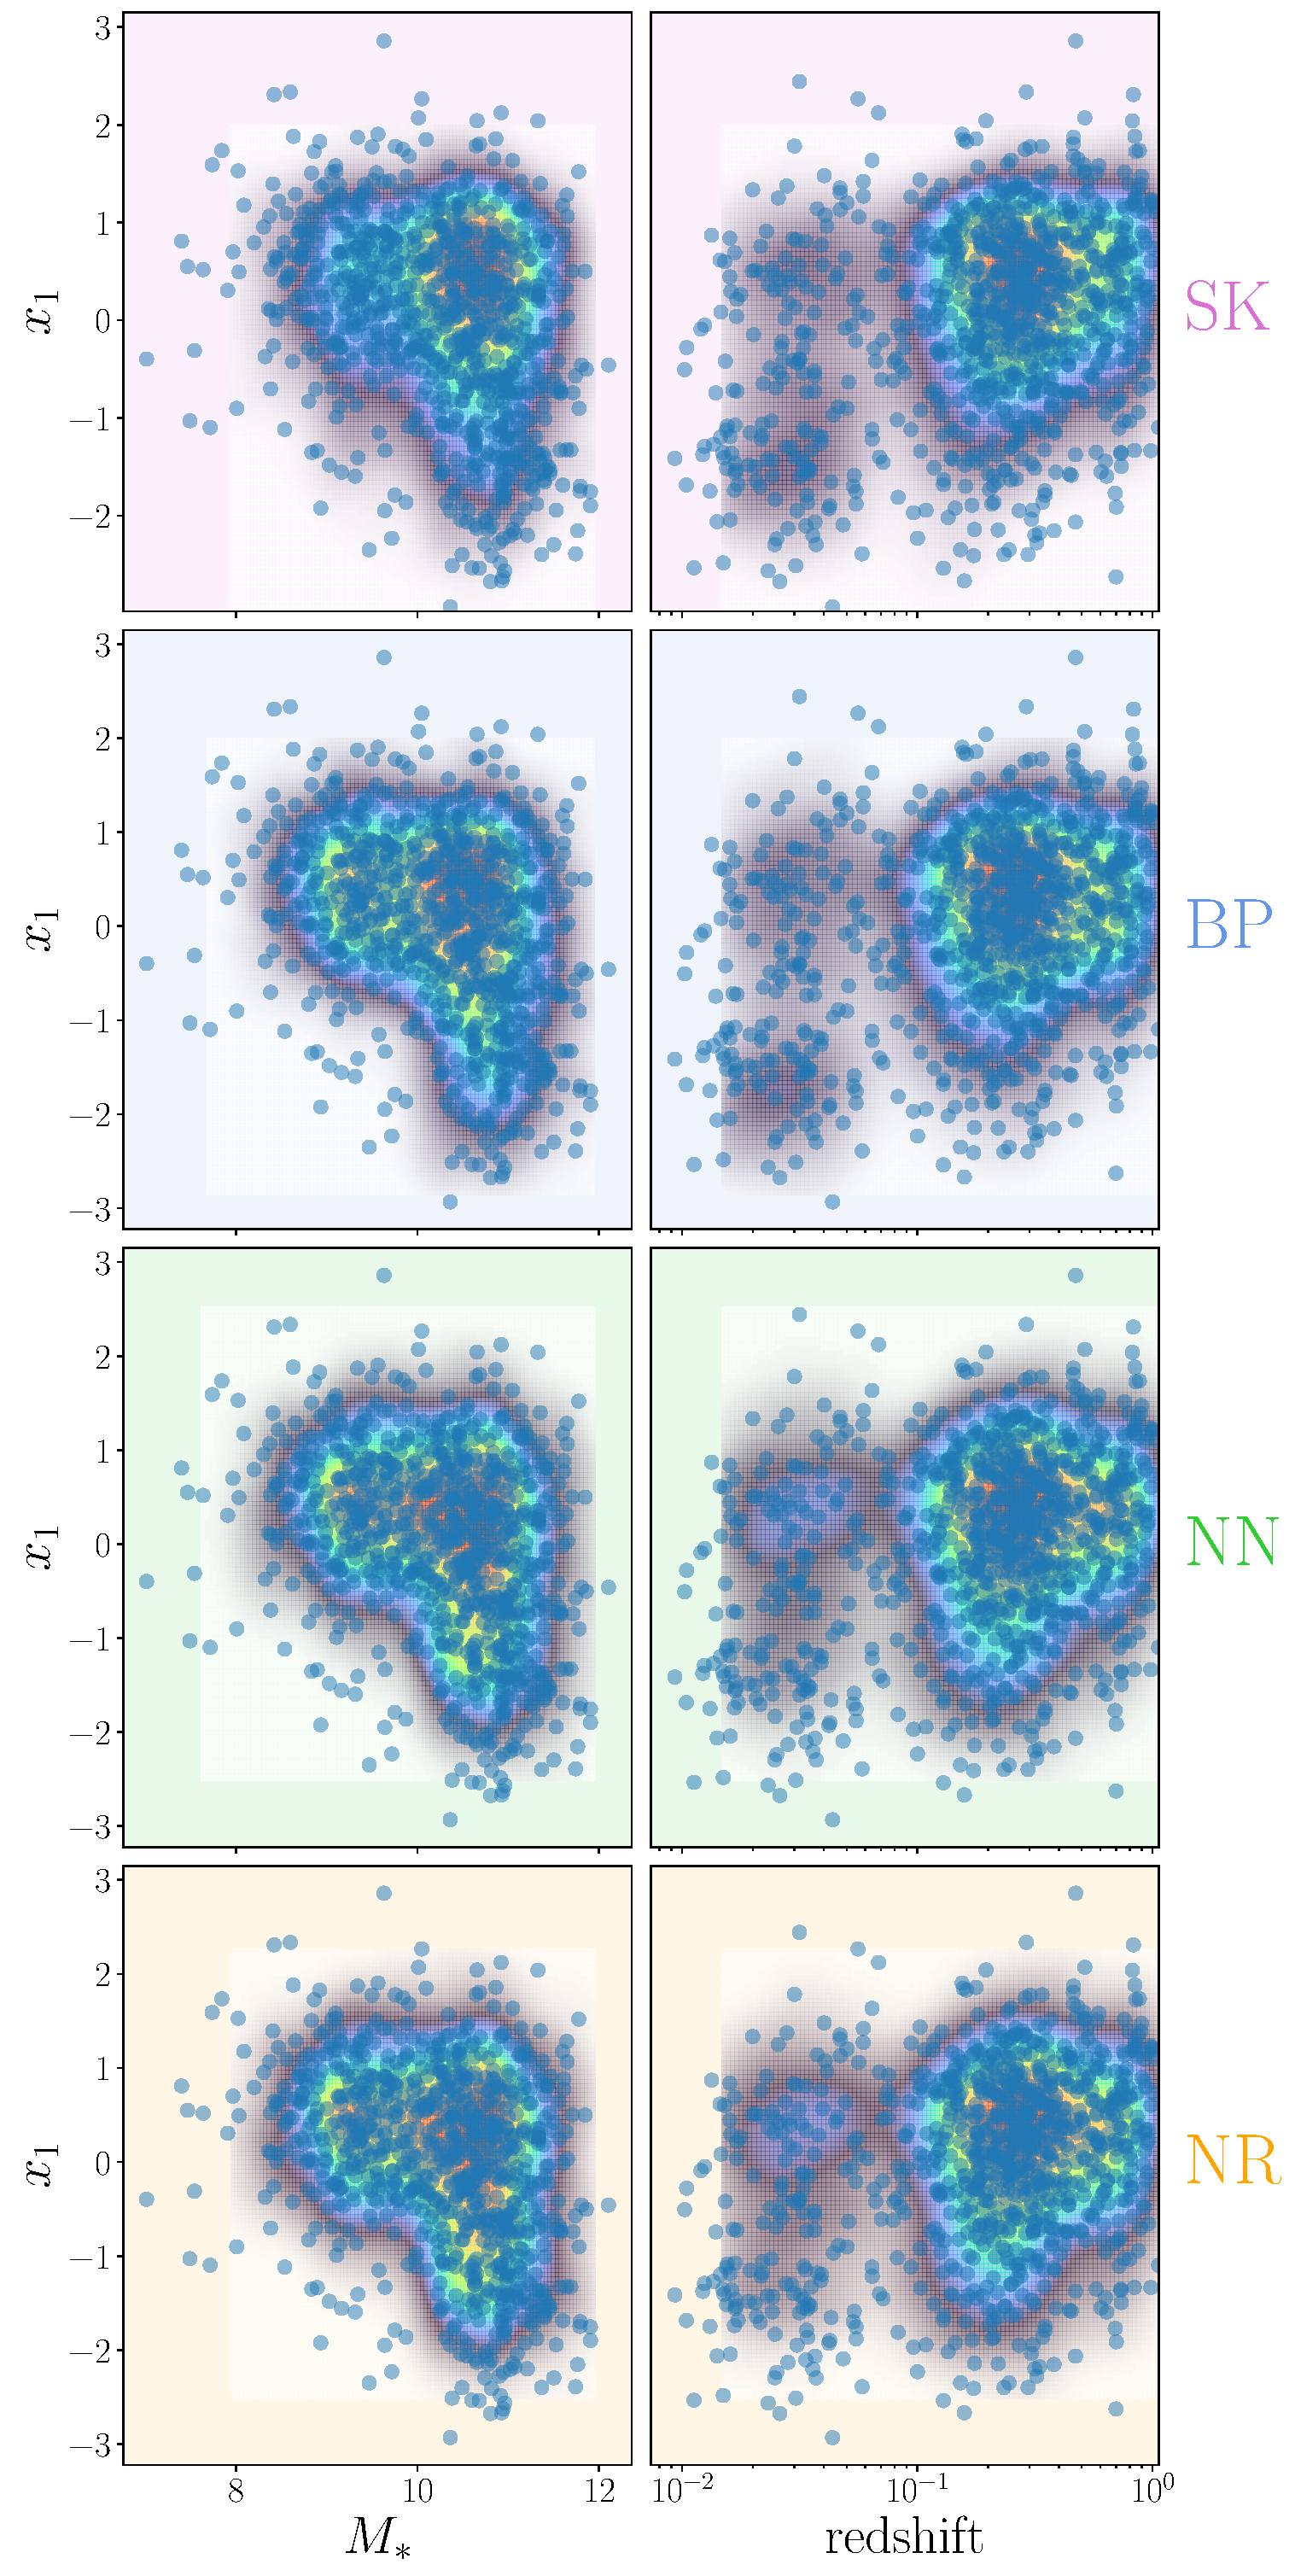
\includegraphics[width=.8\linewidth]{FULL-SNFSUPP_all_RS-MS_kernels}
    \caption[Ajustement en 2D pour tous les modèles]{Accord données réelles et
    simulées en 2D pour tous les modèles.}
    \label{fig:2dhexall}
\end{figure}

\clearpage

\thispagestyle{plain}
% \vspace*{-3cm}
\vfill
\minilof
\vfill
\minilot
\vfill

\bibliographystyle{../main/aa_url}
\shorthandoff{:}
\bibliography{../chapters/99_references}

\end{document}
